% !TEX root = ./rapport.tex
\chapter{Sprints 6 et 7~: Projets, Évaluation, Recrutement, Reporting et Analytique Décisionnelle}

\noindent\textbf{Plan}
\begin{enumerate}
  \item Introduction
  \item Sprint 6~: Projets, tâches, évaluation des performances et recrutement
  \item Sprint 7~: Reporting JasperReports et analytique décisionnelle
  \item Conclusion
\end{enumerate}

% ─────────────────────────────────────────────────────────────
\section{Introduction}
% ─────────────────────────────────────────────────────────────

Cette troisième et dernière release complète la plateforme Synapse par deux
dimensions complémentaires. Le sprint~6 introduit la gestion collaborative des projets et des tâches,
un module d’évaluation des performances par campagnes périodiques, et un
pipeline de recrutement complet intégrant le scoring de CV par IA. Le sprint~7 apporte la dimension décisionnelle~:
génération de rapports JasperReports en PDF et Excel, tableaux de bord analytiques
multi-rôles et module de prédiction de l’attrition.

% ─────────────────────────────────────────────────────────────
\section{Sprint 6~: Projets, tâches, évaluation des performances et recrutement}
% ─────────────────────────────────────────────────────────────

\subsection{Objectifs du sprint}

Le sprint~6 est le sprint à la plus haute densité fonctionnelle du projet~: il
couvre la gestion collaborative des projets et des tâches, l’évaluation des
performances et le pipeline de recrutement avec scoring IA. Ces quatre composants
partagent le même microservice (\textit{projets-service}) et les mêmes entités JPA,
ce qui justifie leur regroupement dans une même itération. La durée est de
\textbf{2 semaines} (13--26 avr. 2026).

\begin{table}[H]
\centering
\caption{Objectifs du sprint 6}
\label{tab:sprint6_obj}
\begin{tabularx}{\textwidth}{VlVLVlVlV}
\rowcolor{headerblue!55}
\hline
\textbf{Tâche} & \textbf{Objectif} & \textbf{US} & \textbf{Estim.} \\
\hline
projets-service & Créer, affecter des membres, suivre l’avancement par agrégation des tâches & US-21 & 2j \\
\hline
taches-service & CRUD des tâches avec statuts, priorités et échéances~; affectation aux membres & US-22, 23 & 2j \\
\hline
Calcul de progression & Recalculer \texttt{PROGRESS\_PCT} à chaque changement de statut d’une tâche & US-23 & 1j \\
\hline
Module d’évaluation & Créer des campagnes d’évaluation, permettre l’auto-évaluation, l’évaluation chef et la validation RH & US-26 & 2j \\
\hline
Pipeline de recrutement & Publication d’offres, candidature publique, scoring IA, shortlisting, entretiens & US-24, 25 & 2j \\
\hline
CvScoringService & Scorer automatiquement les CV candidats via l’API Groq & US-25 & 1j \\
\hline
Interface Angular & Vue projets, tâches, évaluations, pipeline de recrutement & US-21 à 26 & 2j \\
\hline
\end{tabularx}
\end{table}

\subsection{Conception UML}

\subsubsection*{Cas d’utilisation~: Gérer un projet}

La figure~\ref{fig:uc_projet} ci-dessous présente le diagramme de cas d’utilisation
raffiné relatif à la gestion des projets.

% Insert figure: Diagramme de cas d’utilisation raffiné — Gérer un projet
\begin{figure}[H]
  \centering
  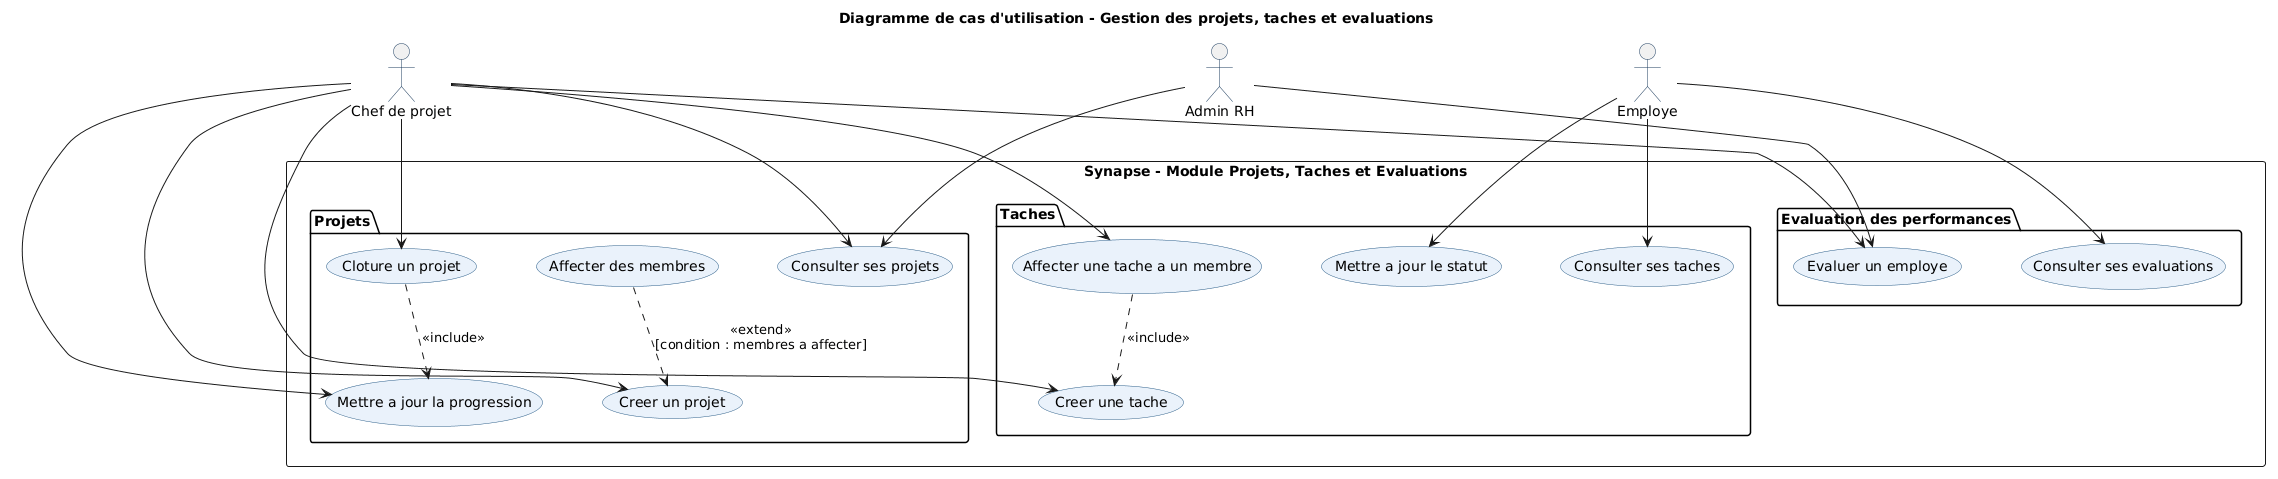
\includegraphics[width=0.90\textwidth,height=0.58\textheight,keepaspectratio]{diagrams/uc_projets_taches_chef.png}
  \caption{Diagramme de cas d’utilisation raffiné~: gestion des projets et des tâches}
  \label{fig:uc_projet}
\end{figure}

La figure~\ref{fig:seq_projet} ci-dessous présente le diagramme de séquence du
cas d’utilisation « Créer un projet et affecter des membres ».


\begin{figure}[H]
  \centering
  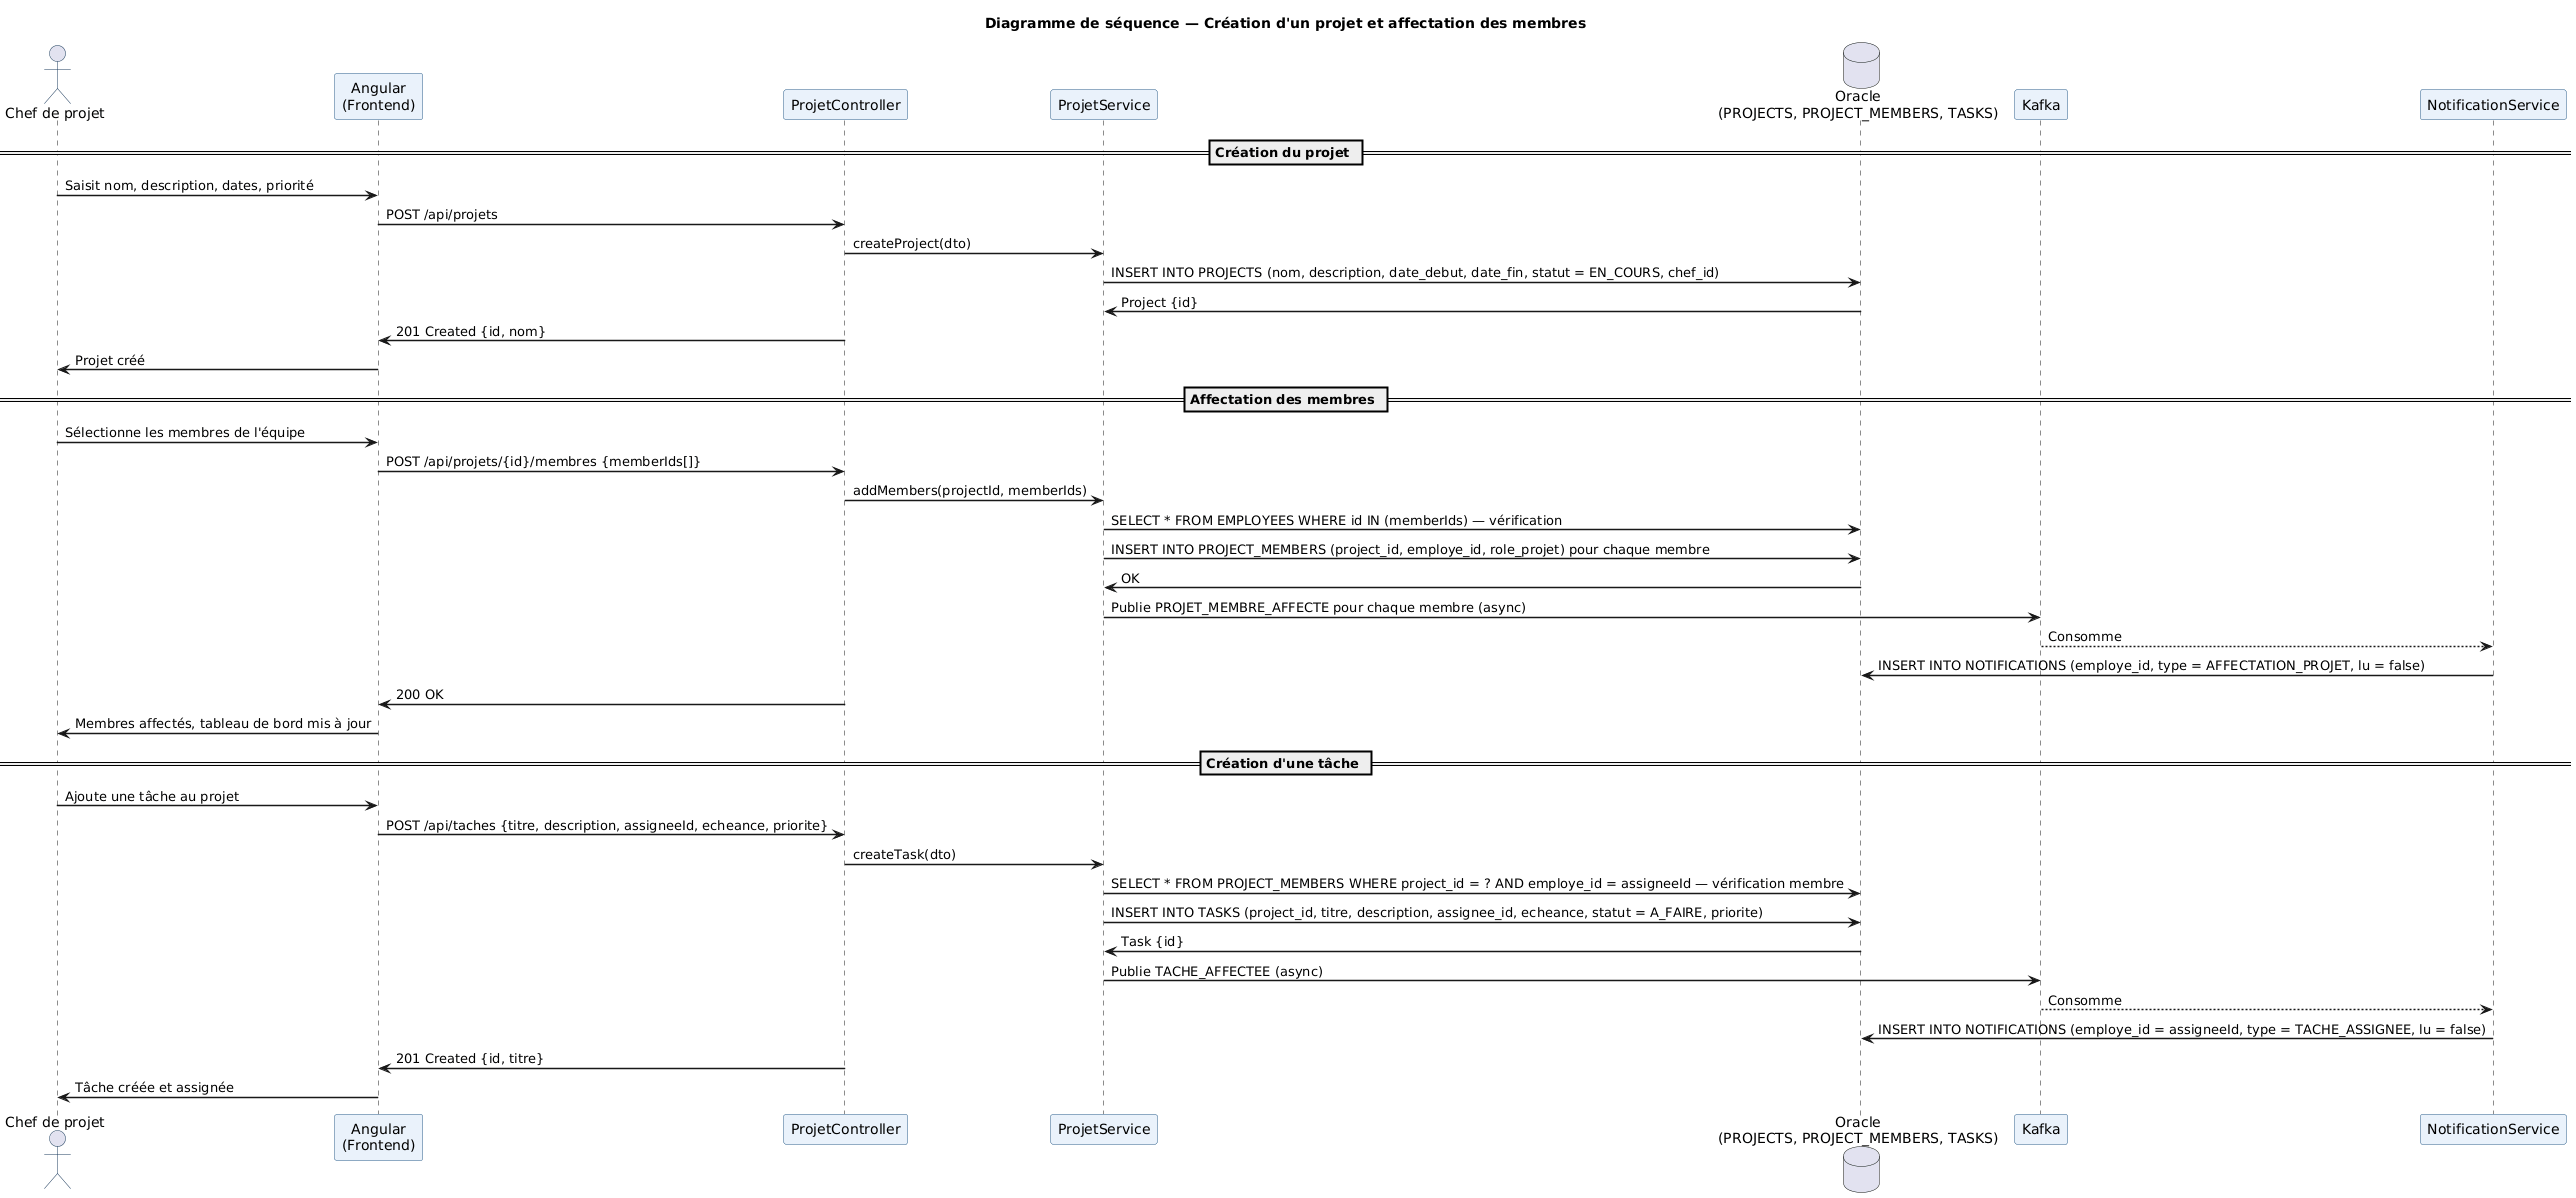
\includegraphics[width=\textwidth,height=0.50\textheight,keepaspectratio]{diagrams/seq_creer_projet.png}
  \caption{Diagramme de séquence~: création d’un projet et affectation des membres}
  \label{fig:seq_projet}
\end{figure}


La figure~\ref{fig:class_projets} ci-dessous présente le diagramme de classes du
domaine projets, tâches, évaluations et recrutement, correspondant aux entités JPA
du \textit{projets-service} et du \textit{taches-service} livrées dans ce sprint.

\begin{figure}[H]
  \centering
  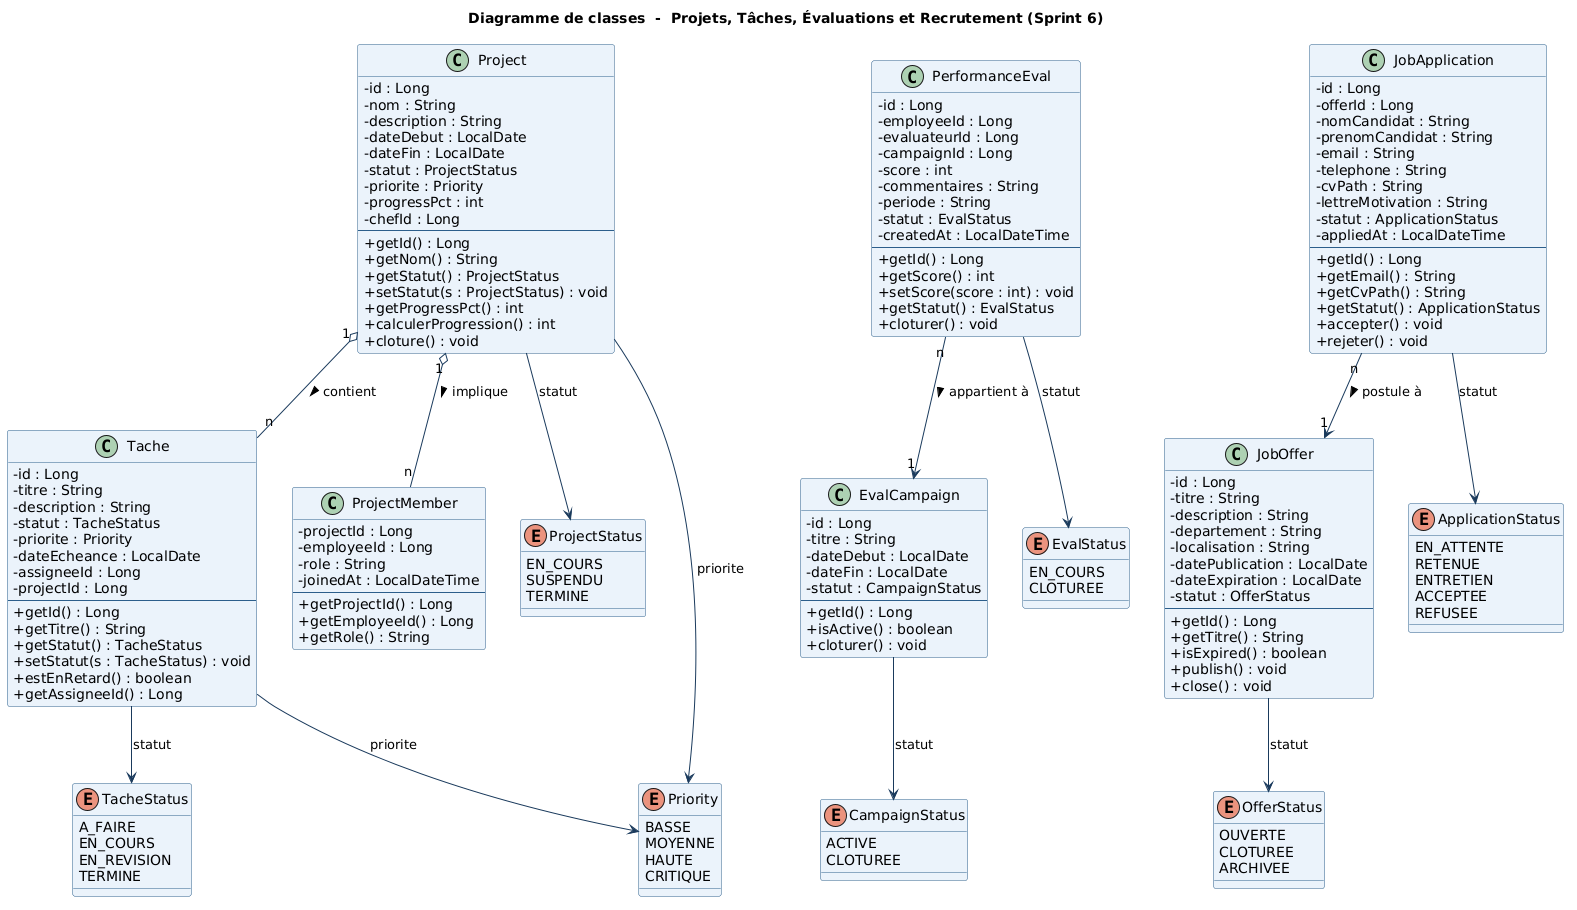
\includegraphics[width=\textwidth,height=0.58\textheight,keepaspectratio]{diagrams/uml_class_projets.png}
  \caption{Diagramme de classes~: domaine projets, tâches, évaluations et recrutement (Sprint 6)}
  \label{fig:class_projets}
\end{figure}

La table~\ref{tab:uc_projet} ci-dessous présente la description textuelle du cas
d’utilisation « Créer un projet et affecter des membres ».

\begin{table}[H]
\centering
\caption{Description textuelle du cas d’utilisation Créer un projet}
\label{tab:uc_projet}
\begin{tabularx}{\textwidth}{VlVLV}
\rowcolor{headerblue!55}
\hline
\textbf{Champ} & \textbf{Description} \\
\hline
Cas d’utilisation & Créer un projet et affecter des membres \\
\hline
Acteur & Chef de projet (\texttt{CHEF}) \\
\hline
Précondition & Le chef est authentifié et appartient à un département \\
\hline
Postcondition & Projet créé, membres affectés, tableau de bord chef mis à jour \\
\hline
Scénario nominal &
\begin{enumerate}[leftmargin=*,nosep]
  \item Le chef saisit le nom, les dates et la priorité du projet
  \item Le projet est créé avec une progression initiale à 0\,\%
  \item Le chef sélectionne les membres de son équipe à affecter au projet
  \item Les affectations sont enregistrées et le tableau de bord est mis à jour
\end{enumerate} \\
\hline
Scénarios alternatifs &
\begin{itemize}[leftmargin=*,nosep]
  \item Date de fin antérieure à la date de début~: message d’erreur, soumission bloquée
  \item Membre déjà affecté au projet~: doublon ignoré, avertissement affiché
\end{itemize} \\
\hline
\end{tabularx}
\end{table}

\subsubsection*{Cas d'utilisation~: Évaluer un employé}

La table~\ref{tab:uc_evaluation} ci-dessous présente la description textuelle du
cas d'utilisation « Évaluer un employé » au sein d'une campagne périodique.

\begin{table}[H]
\centering
\caption{Description textuelle du cas d'utilisation Évaluer un employé}
\label{tab:uc_evaluation}
\begin{tabularx}{\textwidth}{VlVLV}
\rowcolor{headerblue!55}
\hline
\textbf{Champ} & \textbf{Description} \\
\hline
Cas d'utilisation & Évaluer un employé dans le cadre d'une campagne \\
\hline
Acteurs & Chef de projet (\texttt{CHEF}), Administrateur RH (\texttt{ADMIN\_RH}), Employé (\texttt{EMPLOYE}) \\
\hline
Précondition & Une campagne d'évaluation est active (\texttt{statut = ACTIVE}) pour la période courante \\
\hline
Postcondition & Évaluation validée~; score et commentaires persistés dans \texttt{PERFORMANCE\_EVALS} (statut \texttt{CLOTUREE}) \\
\hline
Scénario nominal &
\begin{enumerate}[leftmargin=*,nosep]
  \item Le service RH ouvre une campagne d'évaluation pour une période donnée
  \item Les fiches d'évaluation sont générées pour les membres de l'équipe
  \item L'employé soumet son auto-évaluation
  \item Le chef complète l'évaluation avec un score et des commentaires
  \item Le service RH valide et clôture l'évaluation~; le score final est enregistré
\end{enumerate} \\
\hline
Scénarios alternatifs &
\begin{itemize}[leftmargin=*,nosep]
  \item Campagne non encore ouverte~: soumission d'évaluation bloquée
  \item Évaluation non soumise~: modifiable jusqu'à la soumission définitive
  \item Campagne clôturée~: aucune nouvelle évaluation acceptée
\end{itemize} \\
\hline
\end{tabularx}
\end{table}

\paragraph{Note sur l'auto-évaluation.}
L'étape d'auto-évaluation (étape~3) a été ajoutée en cours de sprint~6 à la
demande des parties prenantes~; elle ne figure pas dans le backlog initial mais
constitue une extension du scénario nominal validée lors de la sprint review.

\subsubsection*{Cas d'utilisation~: Déclencher un recrutement et présélectionner des candidats}

La table~\ref{tab:uc_recrutement} ci-dessous présente la description textuelle du
cas d'utilisation « Déclencher un recrutement », couvrant le circuit complet de la
demande de recrutement jusqu'à la décision d'entretien.

\begin{table}[H]
\centering
\caption{Description textuelle du cas d'utilisation Déclencher un recrutement}
\label{tab:uc_recrutement}
\begin{tabularx}{\textwidth}{VlVLV}
\rowcolor{headerblue!55}
\hline
\textbf{Champ} & \textbf{Description} \\
\hline
Cas d'utilisation & Déclencher un recrutement et présélectionner des candidats \\
\hline
Acteurs & Chef de projet (\texttt{CHEF}), Administrateur RH (\texttt{ADMIN\_RH}), Candidat (public) \\
\hline
Précondition & Le chef est authentifié et a identifié un besoin en recrutement \\
\hline
Postcondition & Candidats présélectionnés, entretiens planifiés, décisions notifiées par e-mail \\
\hline
Scénario nominal &
\begin{enumerate}[leftmargin=*,nosep]
  \item Le chef soumet une demande de recrutement~; le RH la convertit en offre (description générée par l'IA Groq)
  \item Le RH configure les \textit{killer questions} et les critères de screening
  \item Les candidats postulent publiquement~: upload du CV + réponses (\texttt{POST /api/public/apply})~; les \textit{killer questions} échouées entraînent un rejet immédiat
  \item L'IA score chaque CV (0--100) via \texttt{CvScoringService}~; le RH shortliste automatiquement ou manuellement
  \item Les candidats retenus sont convoqués en entretien~; la décision finale est notifiée par e-mail généré par l'IA
\end{enumerate} \\
\hline
Scénarios alternatifs &
\begin{itemize}[leftmargin=*,nosep]
  \item \textit{Killer question} échouée~: candidature rejetée à la soumission (\texttt{POST /validate-killer})
  \item Aucun candidat retenu~: campagne réouverte ou offre modifiée
  \item Entretien annulé~: statut mis à jour, candidat notifié automatiquement
\end{itemize} \\
\hline
\end{tabularx}
\end{table}

\subsection{Implémentation backend}

\begin{table}[H]
\centering
\caption{Endpoints REST du \textit{projets-service} — Sprint 6}
\label{tab:api_projets_s6}
\begin{tabularx}{\textwidth}{VlVlVLVlV}
\rowcolor{headerblue!55}
\hline
\textbf{Méthode} & \textbf{Endpoint} & \textbf{Description} & \textbf{Rôle} \\
\hline
POST & \texttt{/api/chef/projets} & Créer un projet et affecter des membres & CHEF, ADMIN\_RH \\
\hline
PUT & \texttt{/api/chef/taches/\{id\}/statut} & Mettre à jour le statut d’une tâche & EMPLOYE, CHEF \\
\hline
POST & \texttt{/api/chef/evaluations/bulk} & Créer des fiches d’évaluation en masse & CHEF \\
\hline
PUT & \texttt{/api/rh/evaluations/\{id\}/valider} & Valider l’évaluation au niveau RH & RH, ADMIN\_RH \\
\hline
POST & \texttt{/api/chef/recrutement} & Soumettre une demande de recrutement & CHEF \\
\hline
GET & \texttt{/api/public/jobs} & Consulter les offres d’emploi & Public \\
\hline
POST & \texttt{/api/public/apply} & Postuler (CV + killer questions) & Public \\
\hline
POST & \texttt{/api/admin/candidates/auto-shortlist} & Shortlisting IA par seuil de score & ADMIN\_RH \\
\hline
\end{tabularx}
\end{table}

\begin{equation}
  \text{progression} = \frac{\text{nb tâches avec statut TERMINÉ}}{\text{nb total tâches}} \times 100
  \label{eq:progression}
\end{equation}

La progression du projet est recalculée côté serveur à chaque changement de statut de tâche
selon l’équation~\ref{eq:progression} et persistée dans \texttt{PROGRESS\_PCT}.
Les évaluations suivent un cycle en cinq étapes (\texttt{EN\_ATTENTE} →
\texttt{AUTO\_SOUMISE} → \texttt{VALIDEE\_CHEF} → \texttt{VALIDEE\_RH} →
\texttt{CLOTUREE})~; \texttt{POST /evaluations/bulk} permet au chef de générer
les fiches de toute son équipe en une opération. Le \texttt{CvScoringService}
soumet le CV à l’API Groq et persiste le score (0–100) et la justification dans
\texttt{CANDIDATES}~; le shortlisting reste sous contrôle du recruteur.
\texttt{PublicRateLimitFilter} limite les candidatures à 10/h par IP~;
\texttt{/api/public/apply} est le seul endpoint accessible sans token Keycloak.


\subsection{Interfaces de l’application}

Les figures ci-dessous présentent le tableau de bord projets, la vue des tâches,
l'interface d'évaluation des performances et le pipeline de recrutement avec scores IA.
L'interface d'entretiens (planification et décisions) est présentée en Annexe~III
(voir figure~\ref{fig:interviews_view}).

\begin{figure}[H]
  \centering
  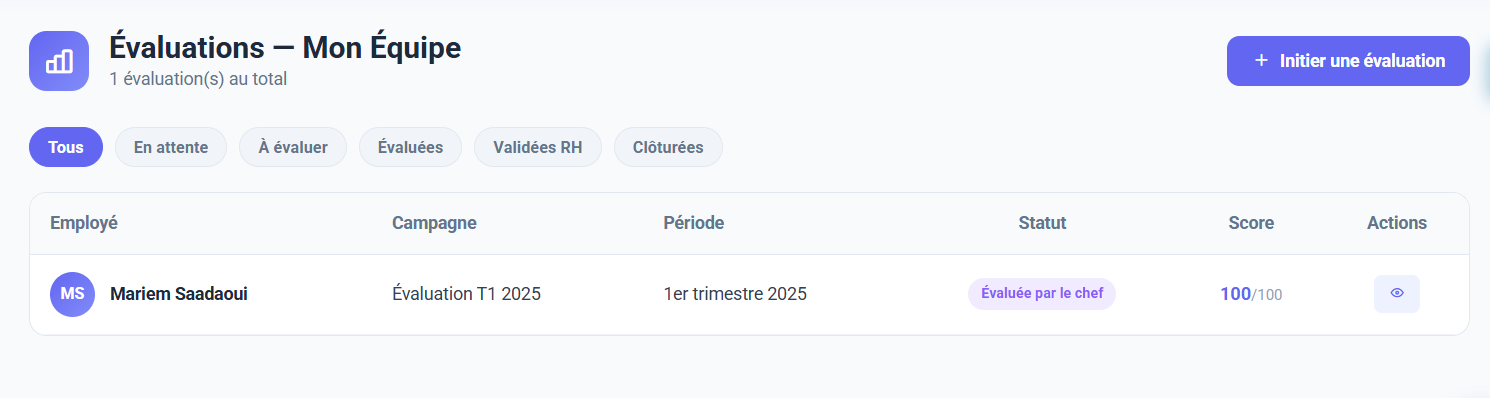
\includegraphics[width=0.82\textwidth,height=0.46\textheight,keepaspectratio]{images/screenshot_evaluations.png}
  \caption{Interface d'évaluation des performances~: campagnes et fiches d'évaluation}
  \label{fig:evaluations_view}
\end{figure}

\begin{figure}[H]
  \centering
  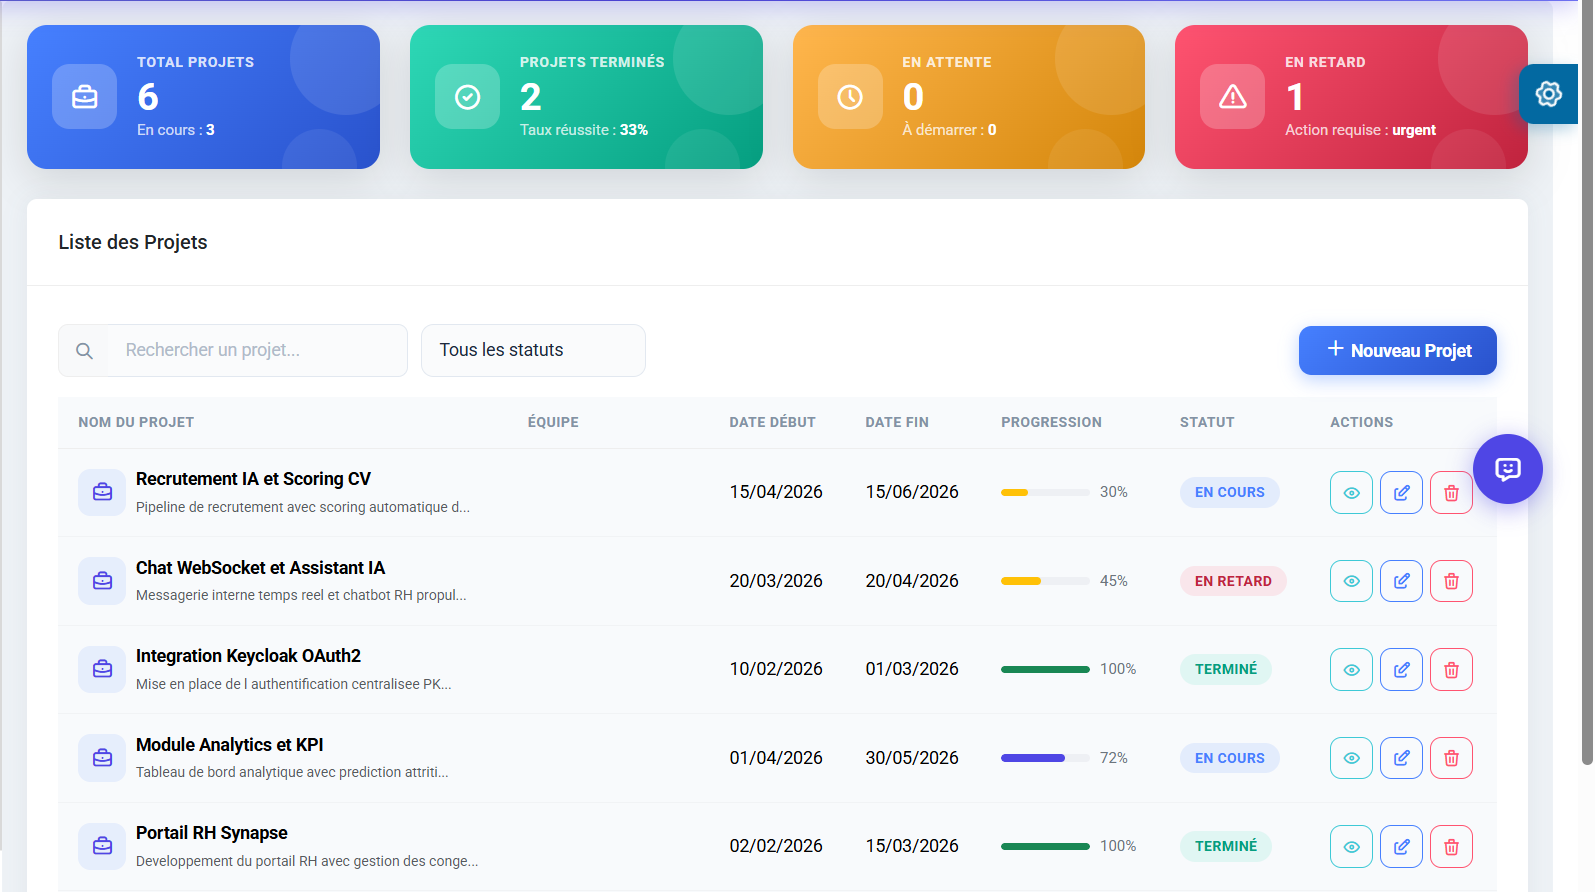
\includegraphics[width=0.82\textwidth,height=0.46\textheight,keepaspectratio]{images/screenshot_projets_list.png}
  \caption{Tableau de bord chef~: liste des projets avec barres de progression}
  \label{fig:projets_list}
\end{figure}

\begin{figure}[H]
  \centering
  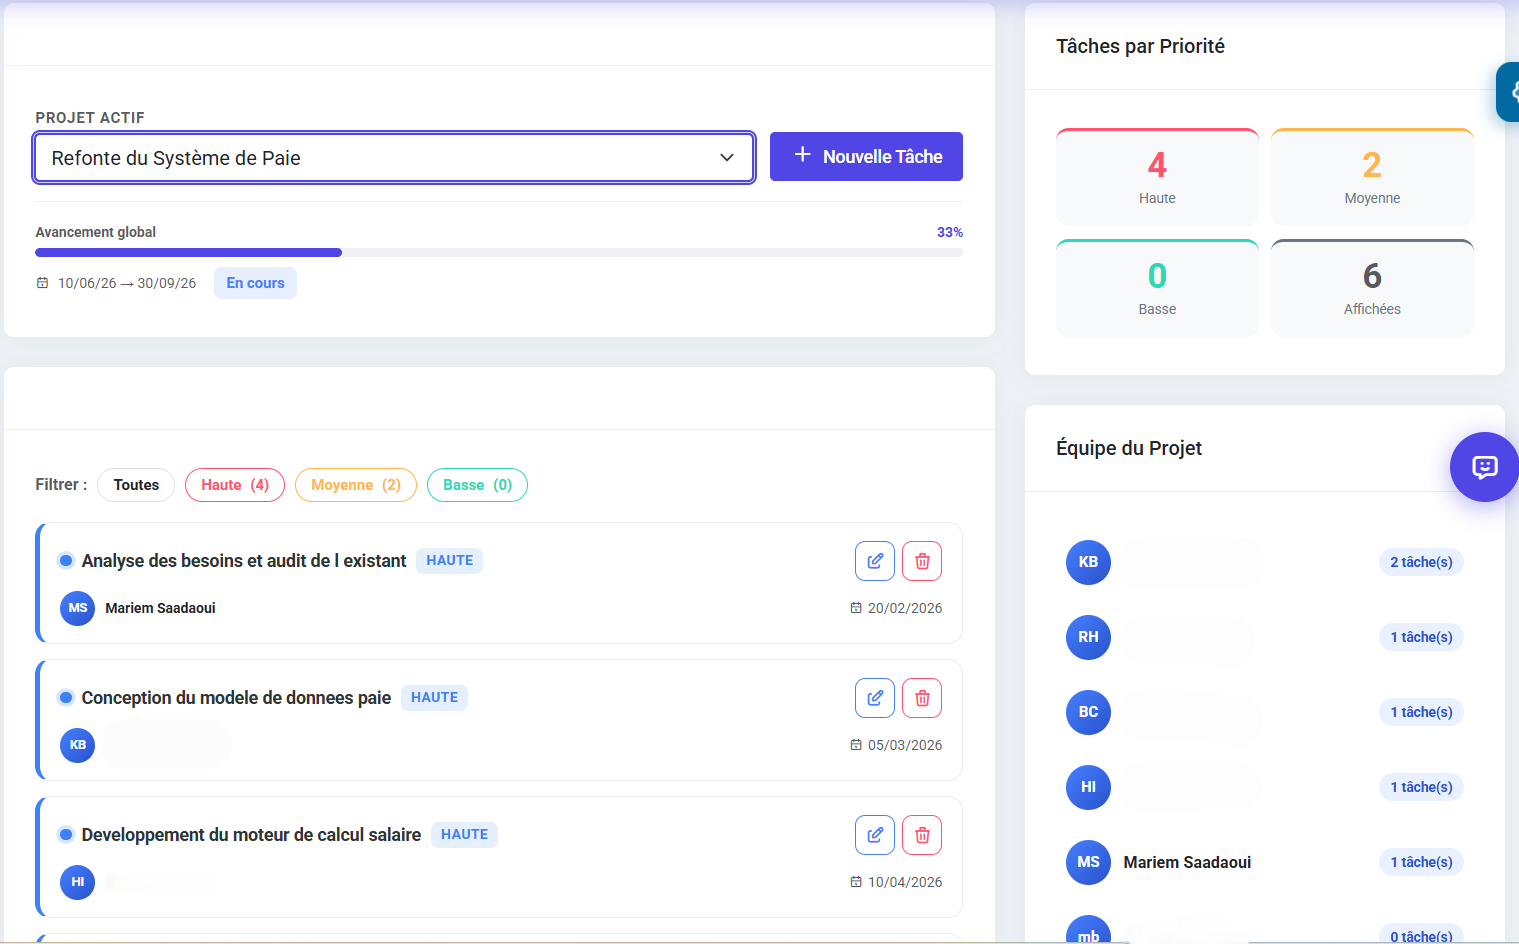
\includegraphics[width=0.82\textwidth,height=0.46\textheight,keepaspectratio]{images/screenshot_taches.png}
  \caption{Gestion des tâches~: statuts (À FAIRE / EN COURS / TERMINÉ) et priorités}
  \label{fig:taches_view}
\end{figure}

\begin{figure}[H]
  \centering
  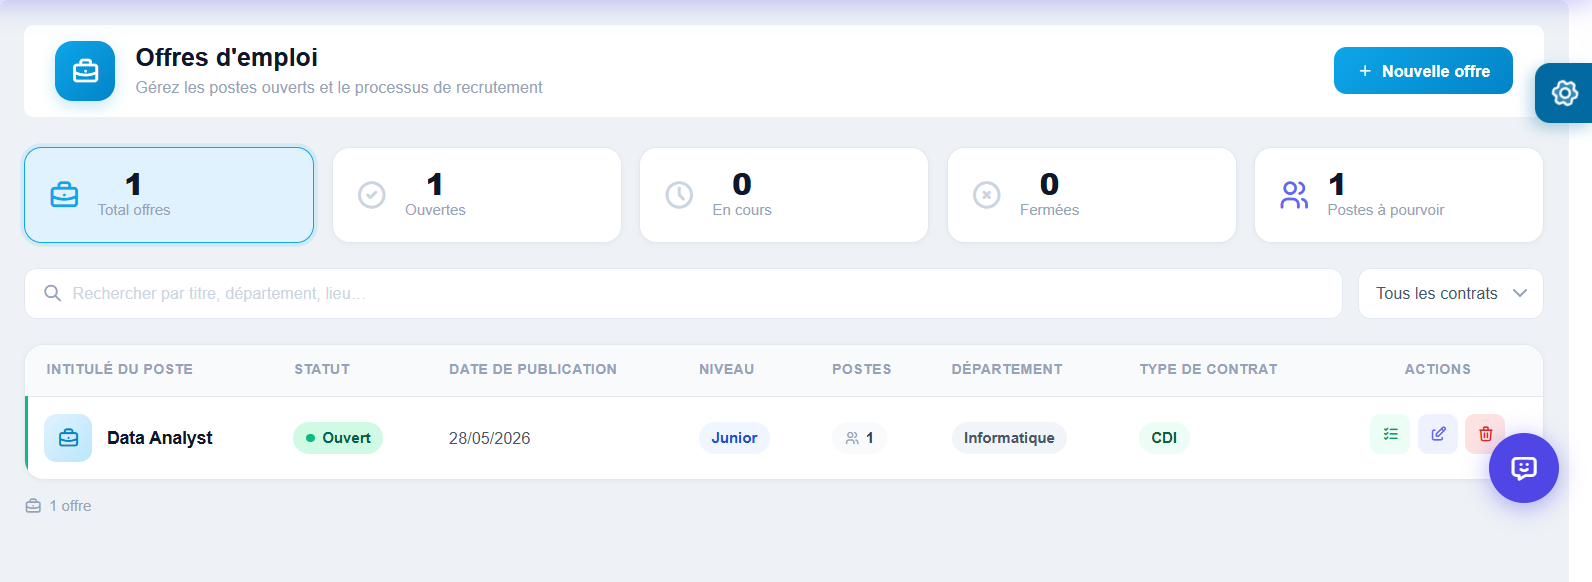
\includegraphics[width=0.82\textwidth,height=0.46\textheight,keepaspectratio]{images/screenshot_job_posting.png}
  \caption{Interface de gestion des offres d'emploi~: publication et paramétrage des questions de présélection}
  \label{fig:job_posting}
\end{figure}

\begin{figure}[H]
  \centering
  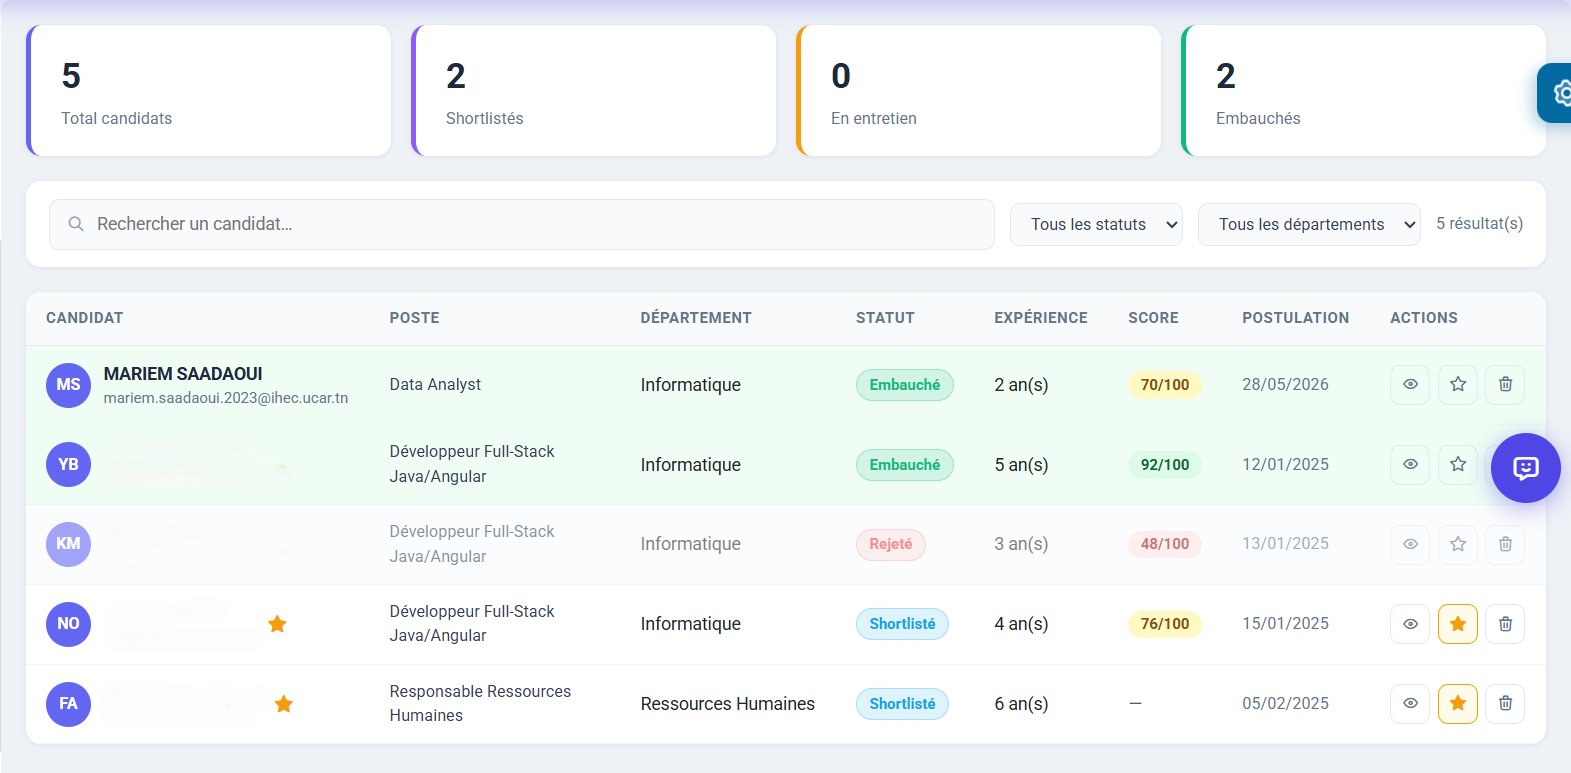
\includegraphics[width=0.82\textwidth,height=0.46\textheight,keepaspectratio]{images/screenshot_candidate_list.png}
  \caption{Interface candidats~: scores IA, shortlisting et gestion du pipeline de recrutement}
  \label{fig:candidate_list}
\end{figure}

\subsection{Implémentation frontend}

\begin{table}[H]
\centering
\caption{Composants Angular — Sprint 6}
\label{tab:angular_sprint6}
\begin{tabularx}{\textwidth}{VlVlVlVLV}
\rowcolor{headerblue!55}
\hline
\textbf{Composant} & \textbf{Route} & \textbf{Rôle} & \textbf{Fonctionnalité} \\
\hline
\texttt{ProjetsComponent} & /chef/projets & CHEF, ADMIN\_RH & Liste des projets avec barres de progression \\
\hline
\texttt{TachesComponent} & /chef/taches & EMPLOYE, CHEF & Kanban de tâches avec mise à jour du statut \\
\hline
\texttt{EvaluationsComponent} & /chef/evaluations & CHEF, RH & Campagnes, auto-évaluation et fiches d'évaluation \\
\hline
\texttt{RecrutementComponent} & /chef/recrutement & CHEF, ADMIN\_RH & Demandes de recrutement et conversion en offre \\
\hline
\texttt{CandidatsComponent} & /admin/candidates & ADMIN\_RH & Scores IA, shortlisting et planification des entretiens \\
\hline
\end{tabularx}
\end{table}

Composants standalone avec stratégie \texttt{OnPush}. L'accès aux routes est
contrôlé par \texttt{requireRoleGuard}~; \texttt{/public/jobs} est la seule route
sans guard. \texttt{ProjetService} expose des observables réactifs consommés par
les composants via \texttt{async pipe}.

\subsection{Sprint review}

\begin{table}[H]
\centering
\caption{Sprint 6 review}
\label{tab:sprint6_review}
\begin{tabularx}{\textwidth}{VLVCVCVCV}
\rowcolor{headerblue!55}
\hline
\textbf{Tâche} & \textbf{Terminé} & \textbf{À améliorer} & \textbf{Inachevé} \\
\hline
projets-service (CRUD + affectation) & \faCheckCircle & & \\
\hline
taches-service (CRUD + statuts) & \faCheckCircle & & \\
\hline
Calcul automatique de progression & \faCheckCircle & & \\
\hline
Module d'évaluation (campagnes + auto-éval + chef + RH) & \faCheckCircle & & \\
\hline
Pipeline de recrutement (offres + candidatures + IA + entretiens) & \faCheckCircle & & \\
\hline
CvScoringService (Groq) + validation score [0--100] + fallback \texttt{-1} & \faCheckCircle & & \\
\hline
Interface Angular~: projets + tâches + évaluations + recrutement & \faCheckCircle & & \\
\hline
\end{tabularx}
\end{table}

\paragraph{Obstacle résolu~: robustesse du parsing JSON Groq.}
Le modèle Groq retournait le score dans des formats variables (bloc \textit{code fence} Markdown, texte superflu)~; deux nettoyages successifs (suppression via regex, extraction du premier objet \texttt{\{...\}}) et une validation de la plage \texttt{[0--100]} ont été implémentés. En cas d'échec ou de score hors plage, \texttt{CvScoringService} retourne \texttt{score = -1} (\texttt{NON\_SCORE}), signalant l'anomalie sans bloquer le pipeline de recrutement.

\section{Sprint 7~: Reporting JasperReports et analytique décisionnelle}
% ─────────────────────────────────────────────────────────────

\subsection{Objectifs du sprint}

Le sprint~7 clôture le développement par la dimension décisionnelle de Synapse~:
génération de rapports PDF/Excel, tableaux de bord analytiques et prédiction
d’attrition. L’objectif est de transformer les données accumulées par les six
sprints précédents en indicateurs exploitables pour la direction. Cette couche analytique dépasse le périmètre des SIRH commerciaux standard,
qui ne proposent pas de prédiction d’attrition intégrée sans module payant. La durée est de
\textbf{2 semaines} (27 avr.--10 mai 2026).

\begin{table}[H]
\centering
\caption{Objectifs du sprint 7}
\label{tab:sprint7_obj}
\begin{tabularx}{\textwidth}{VlVLVlVlV}
\rowcolor{headerblue!55}
\hline
\textbf{Tâche} & \textbf{Objectif} & \textbf{US} & \textbf{Estim.} \\
\hline
analytics-service (JasperReports) & Générer des rapports PDF et Excel depuis les templates \texttt{.jrxml} & US-27, 28 & 3j \\
\hline
Tableaux de bord analytiques & Exposer les KPIs multi-rôles via \texttt{/api/analytics}~; agréger les statistiques de présence dans \texttt{ABSENCE\_STATS} via Kafka consumer & US-29 & 2j \\
\hline
Cache Caffeine & Mettre en cache les résultats analytiques avec TTL de 10 minutes & US-29 & 1j \\
\hline
Prédiction d’attrition & Calculer un score de risque de départ pour chaque employé & US-30 & 2j \\
\hline
Interface Angular & Vue analytics admin/chef, vue attrition, interface de génération de rapports & US-27 à 30 & 2j \\
\hline
\end{tabularx}
\end{table}

% !TEX root = ./rapport.tex
% ══════════════════════════════════════════════════════════════════════
%  ÉTUDE THÉORIQUE — Prédiction de l'attrition
%  Inclus dans chapitre 5 avant le Sprint 7
% ══════════════════════════════════════════════════════════════════════

\subsection{Étude théorique~: Prédiction de l'attrition du personnel}

Lors de l'analyse des besoins du sprint~7, la conception d'un module
capable d'anticiper les départs volontaires s'est imposée~: l'objectif n'était pas de
prédire avec certitude qui allait partir, mais d'identifier les profils présentant
des signaux comportementaux qui, dans la littérature RH, sont associés à une
probabilité de départ plus élevée. Ce module devait être opérationnel dès le
déploiement initial de Synapse, sans historique de départs numérisé.

\subsection{Qu'est-ce que l'attrition~?}

L'attrition désigne le départ non remplacé d'employés d'une organisation. Elle
représente un coût significatif~: au-delà du recrutement, la perte de compétences
accumulées et la baisse de productivité durant la période d'intégration du
remplaçant constituent un coût souvent sous-estimé. Détecter les signaux
précurseurs d'un départ permet d'agir en amont~: entretien de carrière,
revalorisation, ou affectation à un projet plus stimulant.

\subsection{Choix de l'approche~: scoring par règles}

Deux grandes familles d'approches existent pour modéliser l'attrition.

\begin{table}[H]
\centering
\caption{Comparaison des approches de modélisation de l'attrition}
\label{tab:attrition_approaches_theory}
\begin{tabularx}{\textwidth}{|l|L|L|}
\hline
\rowcolor{headerblue!55}
\textbf{Approche} & \textbf{Conditions requises} & \textbf{Application à Synapse} \\
\hline
\rowcolor{rowgray}
Scoring par règles métier & Indicateurs observables, règles connues & \textbf{Retenue}~: applicable dès le déploiement \\
\hline
Machine Learning supervisé & Historique de départs étiquetés (200+ cas minimum) & Perspective~: à envisager après 12--24 mois d'exploitation \\
\hline
\rowcolor{rowgray}
Modèles de survie & Données de durée d'ancienneté complètes & Avancée, non prioritaire \\
\hline
\end{tabularx}
\end{table}

L'approche par machine learning supervisé a été écartée car Arabsoft ne dispose pas, au
moment du déploiement, d'un historique suffisant de départs numérisés pour entraîner
un modèle fiable. Un modèle entraîné sur quelques dizaines d'exemples produirait
des prédictions peu exploitables. L'approche par règles, fondée sur des indicateurs
directement mesurables dans la base Oracle de Synapse, est donc la plus cohérente
avec la réalité du terrain.

\subsection{Facteurs retenus et leur signification}

Les quatre facteurs retenus sont documentés dans la littérature comme des signaux précurseurs de départ\textsuperscript{[26,27]}~: l'\textbf{ancienneté courte} (faible attachement organisationnel)~; un \textbf{volume d'absences élevé} (corrélé à l'insatisfaction)~; un \textbf{taux de rejet élevé des demandes} (perception d'injustice diminuant l'engagement)~; et l'\textbf{absence de projets actifs} (marginalisation professionnelle). Ces quatre indicateurs sont calculables directement depuis les tables Oracle de Synapse (\texttt{EMPLOYEES}, \texttt{LEAVE\_REQUESTS}, \texttt{V\_ALL\_DEMANDES}, \texttt{PROJECT\_MEMBERS}).

\subsection{Limites reconnues}

Ce module produit un score de risque, non une prédiction certifiée. Plusieurs facteurs d'attrition reconnus (rémunération, évolutions de
carrière, dynamique managériale) ne sont pas encore intégrés au schéma de Synapse.
De plus, le scoring est déterministe~: deux employés avec les mêmes indicateurs
obtiennent le même score, sans tenir compte des interactions entre facteurs. Ces
limites sont assumées et définissent la feuille de route naturelle du module~: à
mesure que l'historique s'accumule et que le schéma s'enrichit, une transition vers
un modèle supervisé deviendra viable.


\subsection{Conception UML}

\subsubsection*{Cas d’utilisation~: Générer un rapport}

La figure~\ref{fig:uc_rapport} ci-dessous présente le diagramme de cas d’utilisation
raffiné relatif à la génération de rapports.

% Insert figure: Diagramme de cas d’utilisation raffiné — Générer un rapport
\begin{figure}[H]
  \centering
  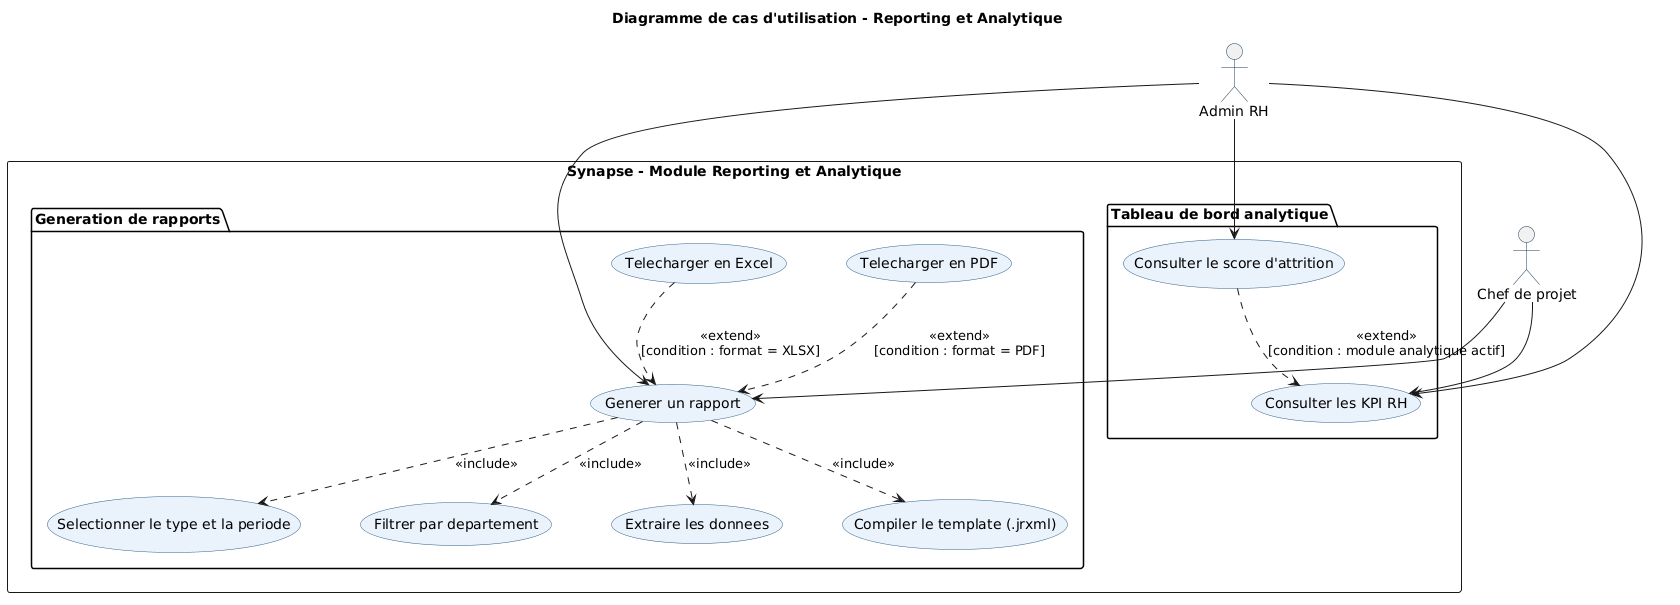
\includegraphics[width=0.90\textwidth,height=0.58\textheight,keepaspectratio]{diagrams/uc_rapport_admin.png}
  \caption{Diagramme de cas d’utilisation raffiné~: génération de rapports JasperReports}
  \label{fig:uc_rapport}
\end{figure}

La figure~\ref{fig:seq_report} ci-dessous présente le diagramme de séquence du cas
d’utilisation «~Générer un rapport PDF~».


\begin{figure}[H]
  \centering
  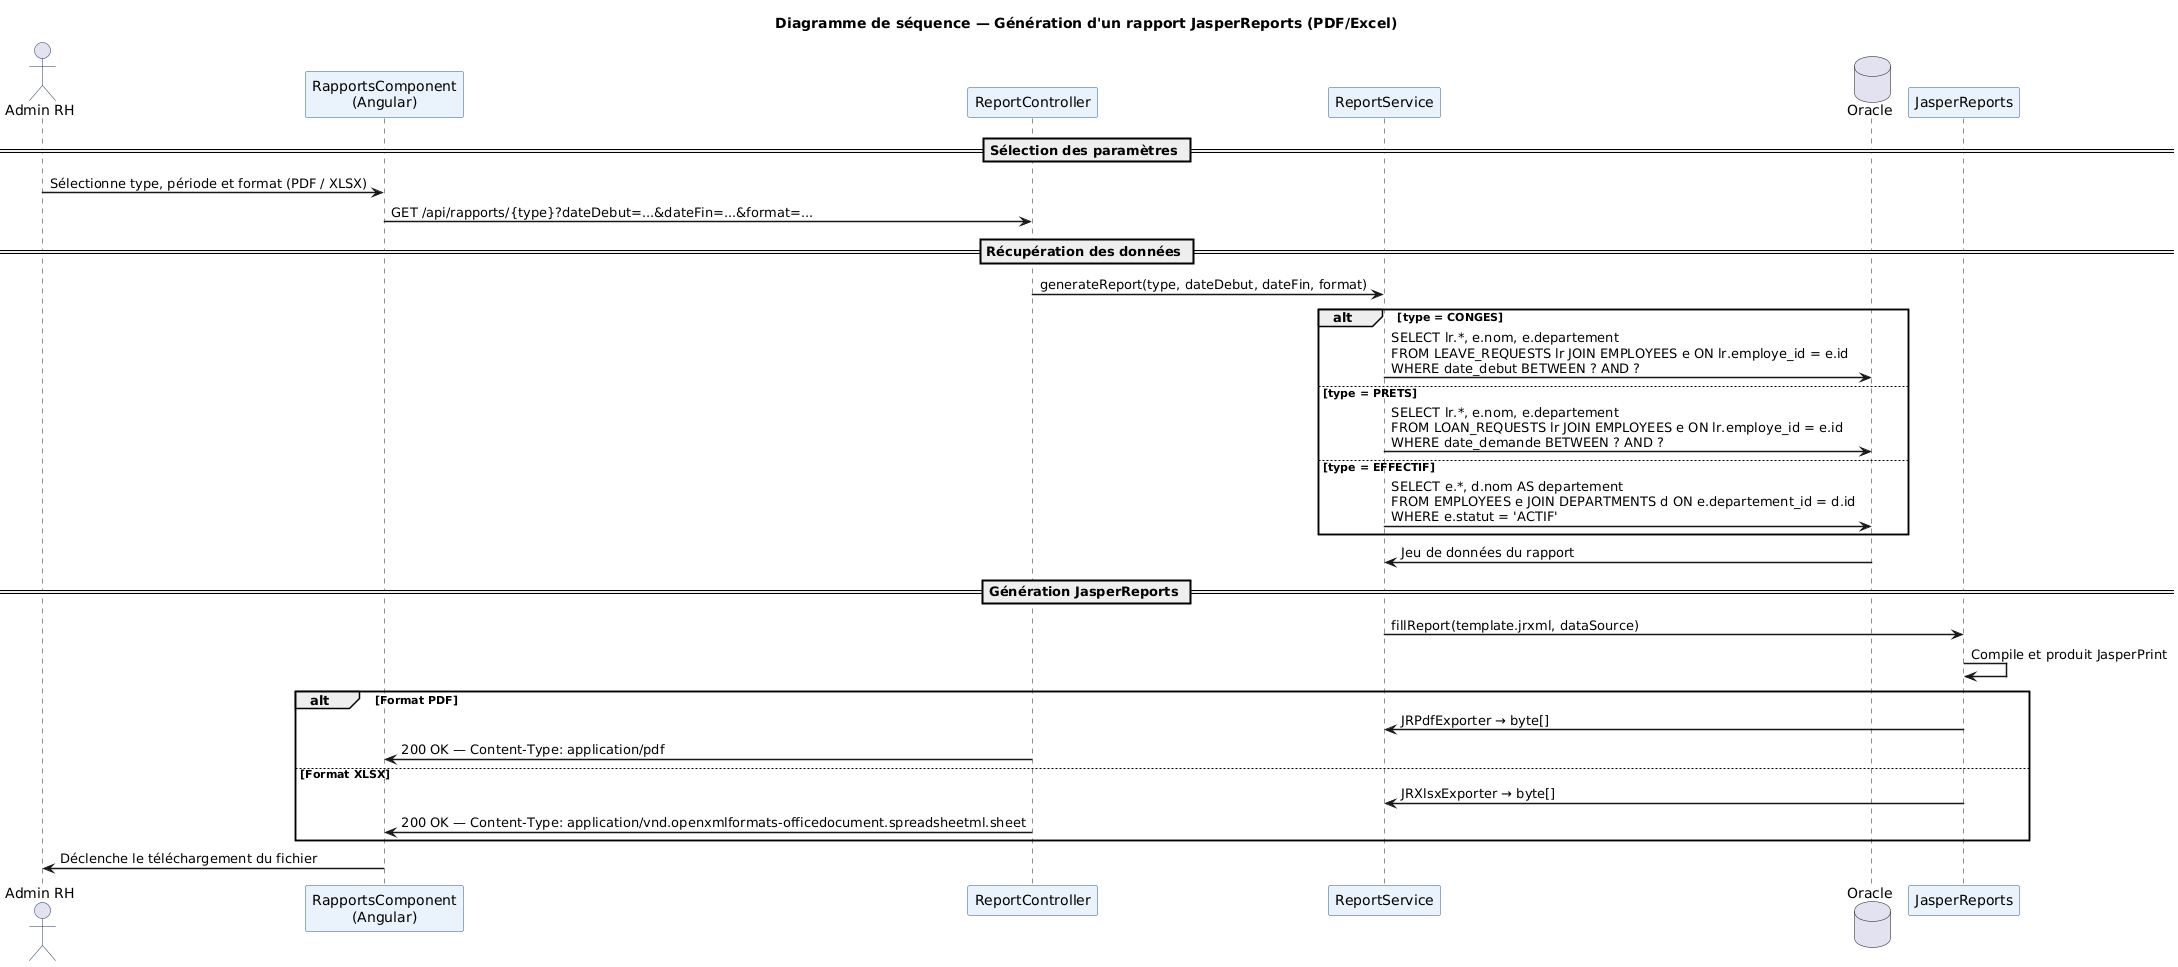
\includegraphics[width=\textwidth,height=0.50\textheight,keepaspectratio]{diagrams/seq_generer_rapport.png}
  \caption{Diagramme de séquence~: génération d’un rapport JasperReports (PDF/Excel)}
  \label{fig:seq_report}
\end{figure}


La table~\ref{tab:uc_rapport} ci-dessous présente la description textuelle du cas
d’utilisation « Générer un rapport ».

\begin{table}[H]
\centering
\caption{Description textuelle du cas d’utilisation Générer un rapport}
\label{tab:uc_rapport}
\begin{tabularx}{\textwidth}{VlVLV}
\rowcolor{headerblue!55}
\hline
\textbf{Champ} & \textbf{Description} \\
\hline
Cas d’utilisation & Générer un rapport \\
\hline
Acteurs & Administrateur RH (\texttt{ADMIN\_RH}), gestionnaire RH (\texttt{RH}), chef de projet (\texttt{CHEF}) \\
\hline
Précondition & L’utilisateur est authentifié et accède à l’interface de reporting \\
\hline
Postcondition & Fichier PDF ou Excel téléchargé dans le navigateur \\
\hline
Scénario nominal &
\begin{enumerate}[leftmargin=*,nosep]
  \item L’utilisateur choisit le type de rapport, la période et le format souhaité (PDF ou Excel)
  \item Le système identifie automatiquement le périmètre de données autorisé selon le profil de l’utilisateur connecté
  \item Les données correspondantes sont collectées et le rapport est généré
  \item Le fichier est mis à disposition et le téléchargement démarre automatiquement dans le navigateur
\end{enumerate} \\
\hline
Scénarios alternatifs &
\begin{itemize}[leftmargin=*,nosep]
  \item Aucune donnée disponible pour la période choisie~: un rapport vide est généré avec un message explicatif
  \item Le service est momentanément indisponible~: un message d’erreur s’affiche et l’utilisateur peut réessayer
\end{itemize} \\
\hline
\end{tabularx}
\end{table}

\subsubsection*{Diagramme de classes~: analytique et attrition}

Le diagramme de la figure~\ref{fig:class_analytics} présente les entités introduites
au sprint~7. \texttt{AttritionPrediction} stocke les quatre facteurs calculés et le
score agrégé pour chaque employé. \texttt{AbsenceStat} matérialise les statistiques
mensuelles agrégées par le consommateur Kafka. Les interfaces \texttt{AnalyticsController}
et \texttt{ReportController} exposent ces données au frontend Angular.

\begin{figure}[H]
  \centering
  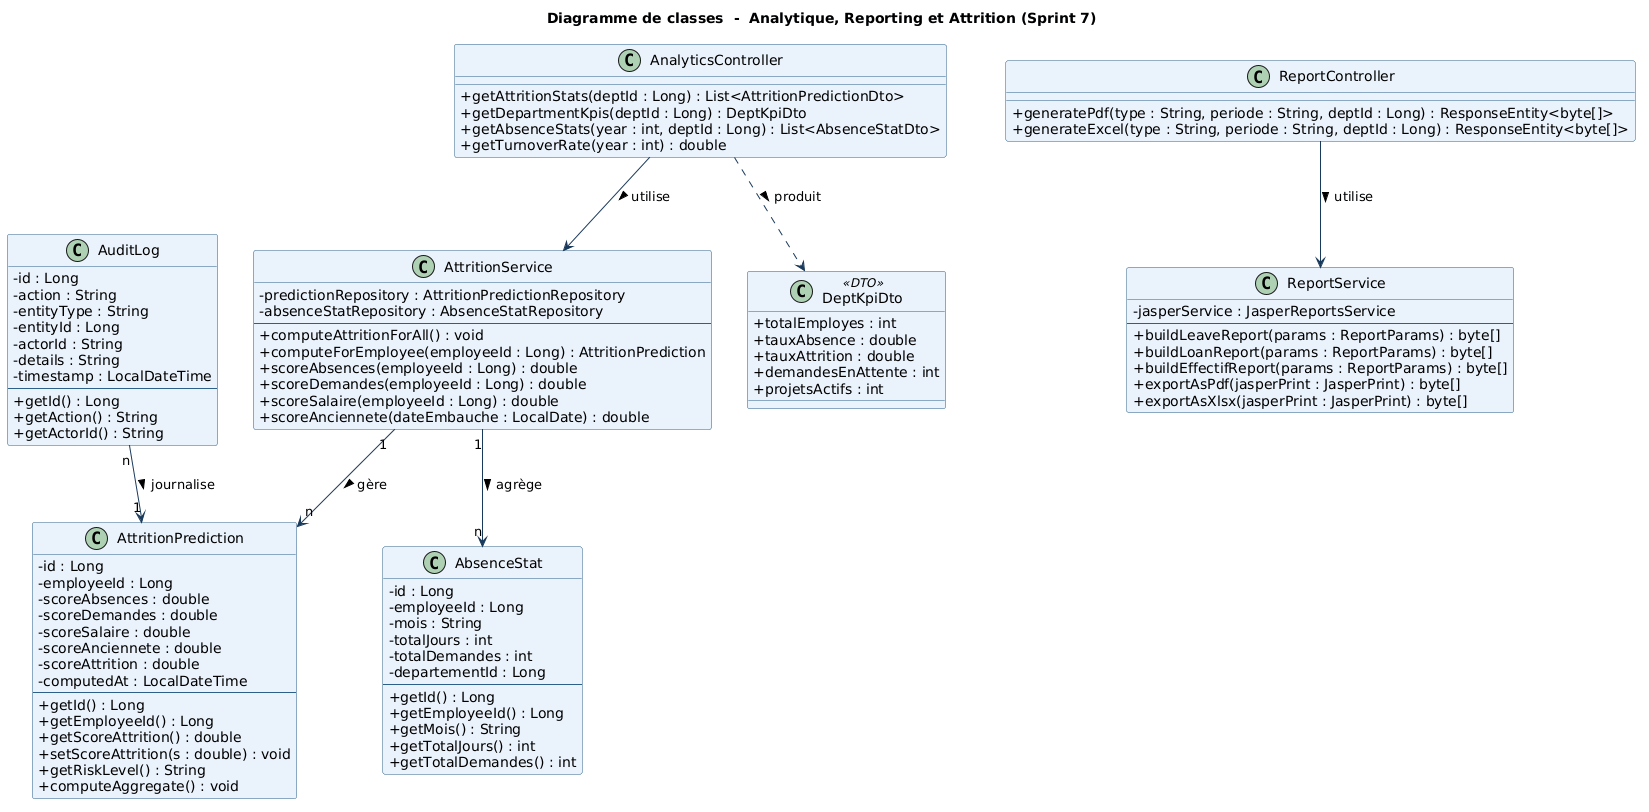
\includegraphics[width=\textwidth,height=0.58\textheight,keepaspectratio]{diagrams/class_sprint7_analytics.png}
  \caption{Diagramme de classes~: domaine analytique, reporting et attrition (Sprint 7)}
  \label{fig:class_analytics}
\end{figure}

\subsection{Modélisation de l’algorithme d’attrition}

Le module de prédiction calcule un score de risque de départ (0--100) pour chaque
employé actif en agrégeant quatre facteurs mesurables, chacun contribuant
au maximum 25 points.

\begin{table}[H]
\centering
\caption{Facteurs de calcul du score d’attrition}
\label{tab:attrition_factors}
\begin{tabularx}{\textwidth}{VlVLVCV}
\rowcolor{headerblue!55}
\hline
\textbf{Facteur} & \textbf{Condition de risque élevé} & \textbf{Points max} \\
\hline
Ancienneté & Embauché depuis moins de 6 mois & 25 \\
\hline
Volume d’absences & $\geq 30$ jours approuvés sur 12 mois & 25 \\
\hline
Taux de rejet & $\geq 50\,\%$ des demandes refusées sur 12 mois & 25 \\
\hline
Engagement projets & Aucun projet actif assigné & 25 \\
\hline
\end{tabularx}
\end{table}

\begin{equation}
  \text{score}_{\text{attrition}} = \text{pts}_{\text{ancienneté}} + \text{pts}_{\text{absences}}
                           + \text{pts}_{\text{refus}} + \text{pts}_{\text{engagement}}
  \label{eq:attrition}
\end{equation}

\noindent Les seuils de niveau de risque sont~:
$\text{ELEVE} \geq 70$, $\text{MOYEN} \in [40, 70[$, $\text{FAIBLE} < 40$.

Le diagramme d'activité ci-dessous modélise le flux algorithmique complet~:
vérification du cache Caffeine, exécution de la requête Oracle, calcul parallèle
des quatre facteurs, application de la formule de scoring et classification par
niveau de risque.

\begin{figure}[H]
  \centering
  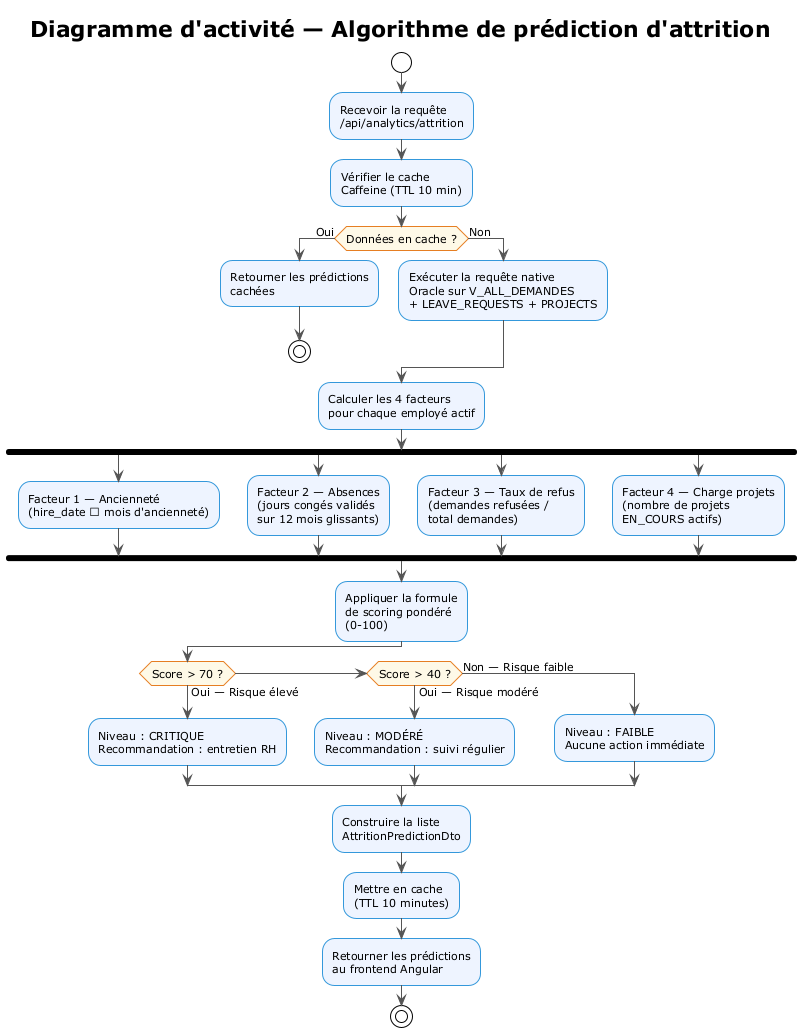
\includegraphics[width=0.80\textwidth,height=0.62\textheight,keepaspectratio]{images/activity_attrition.png}
  \caption{Diagramme d'activité~: algorithme de prédiction d'attrition (cache → Oracle → scoring → classification)}
  \label{fig:activity_attrition}
\end{figure}

\subsection{Implémentation backend}

\begin{table}[H]
\centering
\caption{Endpoints REST de l'\textit{analytics-service} — Sprint 7}
\label{tab:api_analytics_s7}
\begin{tabularx}{\textwidth}{VlVlVLVlV}
\rowcolor{headerblue!55}
\hline
\textbf{Méthode} & \textbf{Endpoint} & \textbf{Description} & \textbf{Rôle} \\
\hline
GET & \texttt{/api/analytics/kpis} & KPIs globaux (absences, effectifs, demandes) & RH, ADMIN\_RH, CHEF \\
\hline
GET & \texttt{/api/reports/generate} & Générer un rapport PDF ou Excel (JasperReports) & RH, ADMIN\_RH, CHEF \\
\hline
GET & \texttt{/api/admin/attrition} & Scores de risque de départ par employé & RH, ADMIN\_RH \\
\hline
POST & \texttt{/api/admin/attrition/refresh} & Forcer le recalcul et invalider le cache & ADMIN\_RH \\
\hline
\end{tabularx}
\end{table}

Les résultats analytiques sont mis en cache Caffeine (TTL 10 min) et invalidés via
\texttt{@CacheEvict}. Le périmètre des données est filtré selon le rôle connecté~:
un chef n'accède qu'aux KPIs de son équipe. Les rapports JasperReports sont compilés
en mémoire et renvoyés en \texttt{application/pdf} ou \texttt{application/vnd.ms-excel}.

Les migrations Flyway V6–V11 complètent le schéma~: \texttt{REPORT\_LOGS},
\texttt{AUDIT\_LOGS}, \texttt{ML\_PREDICTIONS} (V6)~; vue \texttt{V\_ALL\_DEMANDES}
(V10)~; données de référence et jeux de démonstration (V7–V9). La table
\texttt{ML\_PREDICTIONS} est conçue pour plusieurs types de prédictions~;
seul \texttt{TURNOVER} (attrition) est implémenté dans cette release. L’\textit{analytics-service}
agrège les facteurs d’attrition via une requête Oracle avec \texttt{LEFT JOIN}
et met les résultats en cache Caffeine (TTL 10 min)~; la table \texttt{ABSENCE\_STATS},
alimentée par un consommateur Kafka, fournit les KPIs de présence sans requête
en temps réel.

\subsection{Interfaces de l’application}

Les figures ci-dessous présentent les interfaces analytiques et de reporting~:
tableau de bord, formulaire de génération, exemple de rapport PDF et détail d'un
profil à risque. La vue principale de prédiction d'attrition (KPI globaux et liste
des employés par score) est présentée en Annexe~IV (voir figure~\ref{fig:attrition_main}).

\begin{figure}[H]
  \centering
  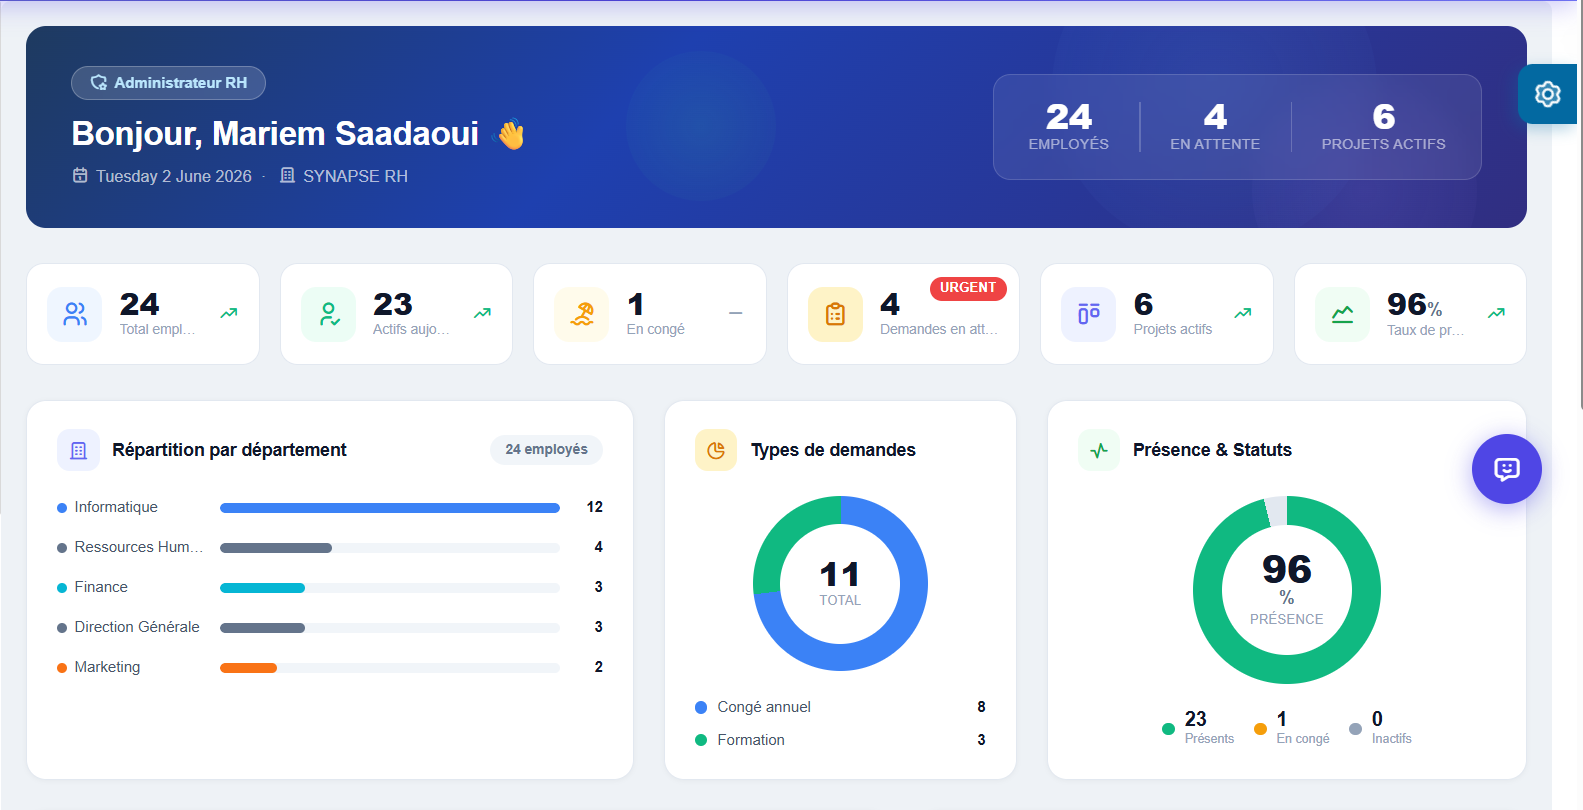
\includegraphics[width=0.82\textwidth,height=0.46\textheight,keepaspectratio]{images/screenshot_admin_dashboard.png}
  \caption{Tableau de bord analytique~: KPIs globaux, graphiques de tendance et top absences}
  \label{fig:analytics_dashboard}
\end{figure}

\begin{figure}[H]
  \centering
  
\includegraphics[width=0.82\textwidth,height=0.46\textheight,keepaspectratio]{images/screenshot_rapports_form.png}
  \caption{Interface de génération de rapports~: sélection du type, du département et du format}
  \label{fig:rapports_form}
\end{figure}

\begin{figure}[H]
  \centering
  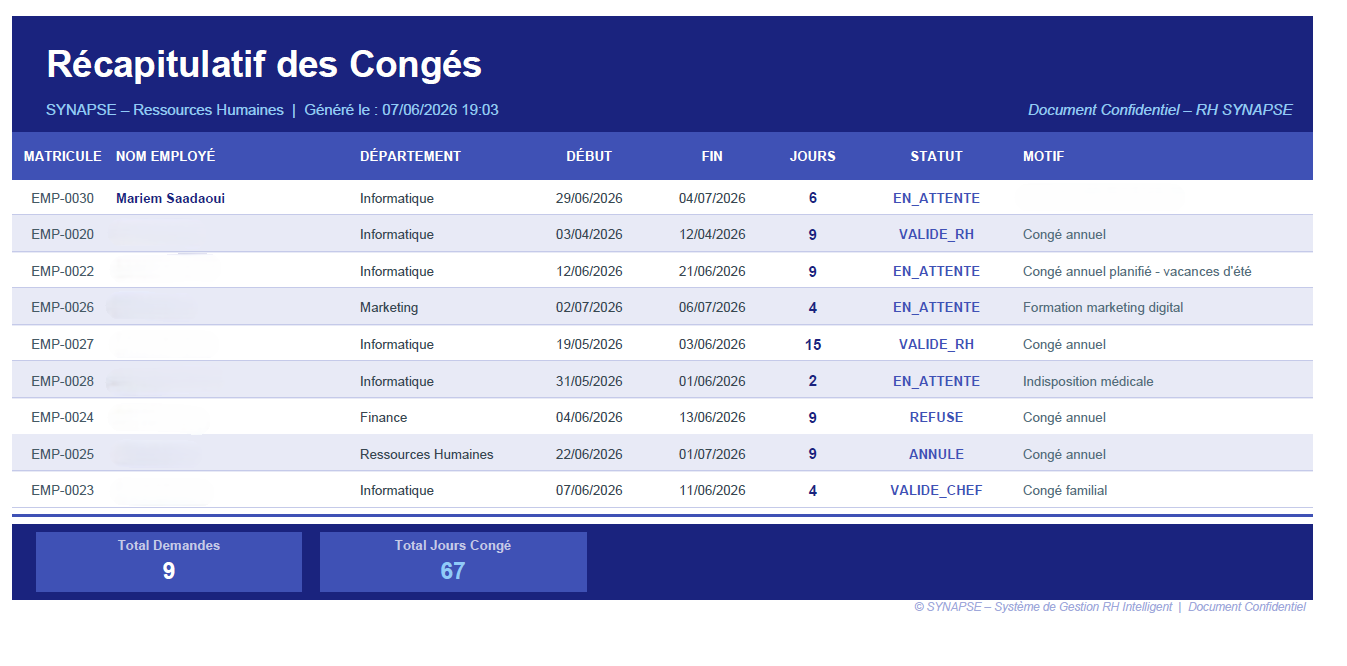
\includegraphics[width=0.82\textwidth,height=0.46\textheight,keepaspectratio]{images/screenshot_rapport_pdf.png}
  \caption{Exemple de rapport PDF généré par JasperReports~: liste des congés par département}
  \label{fig:rapport_pdf}
\end{figure}

\begin{figure}[H]
  \centering
  
\includegraphics[width=0.55\textwidth,keepaspectratio]{images/screenshot_attrition_detail.png}
  \caption{Détail d'un profil à risque élevé~: gauge de score, facteurs et recommandations RH}
  \label{fig:attrition_detail}
\end{figure}

\subsection{Implémentation frontend}

\begin{table}[H]
\centering
\caption{Composants Angular — Sprint 7}
\label{tab:angular_sprint7}
\small
\begin{tabularx}{\textwidth}{V>{\raggedright\arraybackslash}p{4.2cm}VlVlVLV}
\rowcolor{headerblue!55}
\hline
\textbf{Composant} & \textbf{Route} & \textbf{Rôle} & \textbf{Fonctionnalité} \\
\hline
\texttt{Dashboard\-Analytics\-Component} & /admin/analytics & RH, ADMIN\_RH & KPIs globaux, graphiques de tendance et top absences \\
\hline
\texttt{RapportsComponent} & /admin/rapports & RH, ADMIN\_RH, CHEF & Formulaire de génération et téléchargement du rapport \\
\hline
\texttt{AttritionComponent} & /admin/attrition & RH, ADMIN\_RH & Liste des employés triés par score de risque décroissant \\
\hline
\texttt{Attrition\-Detail\-Component} & /admin/attrition/\{id\} & RH, ADMIN\_RH & Gauge de score, facteurs détaillés et recommandations RH \\
\hline
\end{tabularx}
\end{table}

\texttt{AnalyticsService} expose les KPIs via des observables consommés en
\texttt{async pipe} (\texttt{OnPush}). Le téléchargement du rapport utilise
\texttt{responseType: 'blob'} converti en lien dynamique. L'\texttt{AttritionComponent}
code-colore les lignes selon le niveau de risque (\texttt{ELEVE / MOYEN / FAIBLE}).

\subsection{Sprint review}

\begin{table}[H]
\centering
\caption{Sprint 7 review}
\label{tab:sprint7_review}
\begin{tabularx}{\textwidth}{VLVCVCVCV}
\rowcolor{headerblue!55}
\hline
\textbf{Tâche} & \textbf{Terminé} & \textbf{À améliorer} & \textbf{Inachevé} \\
\hline
analytics-service (JasperReports PDF + Excel) & \faCheckCircle & & \\
\hline
Tableaux de bord analytiques multi-rôles & \faCheckCircle & & \\
\hline
Cache Caffeine + invalidation @CacheEvict & \faCheckCircle & & \\
\hline
Module de prédiction d’attrition & \faCheckCircle & & \\
\hline
Interface Angular~: analytics + rapports + attrition (\texttt{OnPush} appliqué) & \faCheckCircle & & \\
\hline
\end{tabularx}
\end{table}

\paragraph{Obstacle résolu~: compatibilité JasperReports/Java~21 et stratégie OnPush.}
L’intégration de JasperReports~6.21.0 sur Java~21 a nécessité d’exclure \texttt{commons-logging} et de cibler l’API \texttt{JRPdfExporter} dans sa version stable. Parallèlement, \texttt{RapportsComponent} manquait la déclaration \texttt{ChangeDetectionStrategy.OnPush} malgré l’injection de \texttt{ChangeDetectorRef}~; cet ajout a éliminé les rendus parasites sur les tableaux de bord multi-graphiques.

% ─────────────────────────────────────────────────────────────
\section{Conclusion}
% ─────────────────────────────────────────────────────────────

Cette dernière release clôture le développement de Synapse en apportant les
fonctionnalités les plus avancées~: gestion collaborative des projets et des tâches,
scoring IA des CV, reporting multi-format via JasperReports, tableaux de bord
analytiques à invalidation événementielle et prédiction de l’attrition fondée sur
quatre indicateurs comportementaux mesurables. L’ensemble des sept sprints planifiés
a été livré sans report au backlog suivant.
